Control Algorithm:



Dentro del Dominio del controlador tendremos Un modelo de lo que significa para nosotros un encoder. Podemos ver en la figura \ref{fig:EncoderInterface} que es una interfaz que actua como puerto de salida hacia la implementación, el adaptador que contemplará el uso de una librería en golang para raspberry que permita la interacción de los pines de lectura con los que está conectado el encoder y realice las operaciones pertinentes para obtener la posición. Todo esto no es responsabilidad del Dominio. No nos atañe el dispositivo en el que se va a ejecutar la lógica de control a partir de este encoder. Simplemente nos interesa que tenga una función de observación que llamaremos \textit{watchdog} de las lectura de dichos pines y una función a la que llamaremos para obtener la posición en el momento que deseemos saberlo \textit{getPosition} También atañe al dominio saber que hay que resetear los parámetros del encoder cuando interese y que hay que desactivar el hardware cuando se deje de utilizar para que no haya inconsistencias a la hora de volver a ejecutar el programa.


\begin{figure}[H]
    \centering
    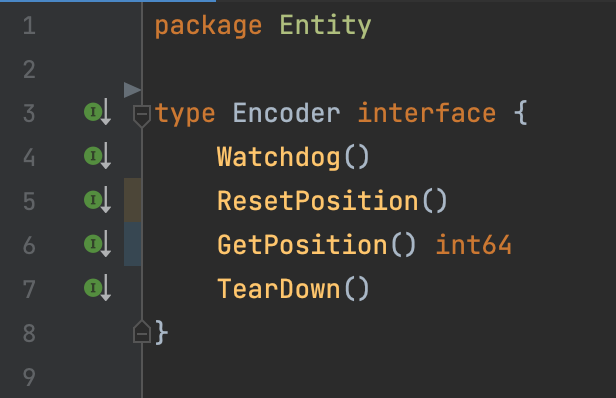
\includegraphics[height=0.2\textheight]{./part/Ejecucion/Seguimiento/PidControl/img/EncoderInterface}
    \caption{Encoder.go}\label{fig:EncoderInterface}
\end{figure}

Pasando a la implementación el punto de más relevancia se encuentra remarcado en rojo en la figura \ref{fig:EncoderAdapter} donde podemos ver que cuando se ejecuta la función de \textit{watchdog} se ponen en marcha dos gorutines; una para vigilar cada lectura de los dos pines del Encoder.

Se queda en un bucle infinito la primera sentencia de dicho bucle es quedarse bloqueado hasta que haya un cambio en el pin de lectura, ya sea de 0 a 1 o de 1 a 0. Si esto ocurre lo primero que hace es bloquear todas las demas gorutines porque va a hacer cambios en memoria de forma atómica, escribe la información de dicha lectura en un array de lecturas y desbloquea las gorutines, se termina y vuelve a esperar.

Independientemente, el watchdog, una vez lanzadas las gorutines de lectura se queda en bucle infinito que lo que hace es bloquear las gorutinas. Extraer un elemento del array de lecturas y procesarlo.

Tal y como están diseñadas la gorutines, se van encolando y esperan su momento en la CPU para ejecutarse. si hay bloqueos también esperan su turno. De esta forma supongamos que el procesado de una lectura tardara más de la cuenta. Se irían encolando las gorutines a la espera de poder añadirse en el array de lecturas, pero no se perderían. De esta forma Se consigue leer exactamente los 360 pulsos por vuelta del encoder sin perder ninguno.

\begin{figure}[H]
    \centering
    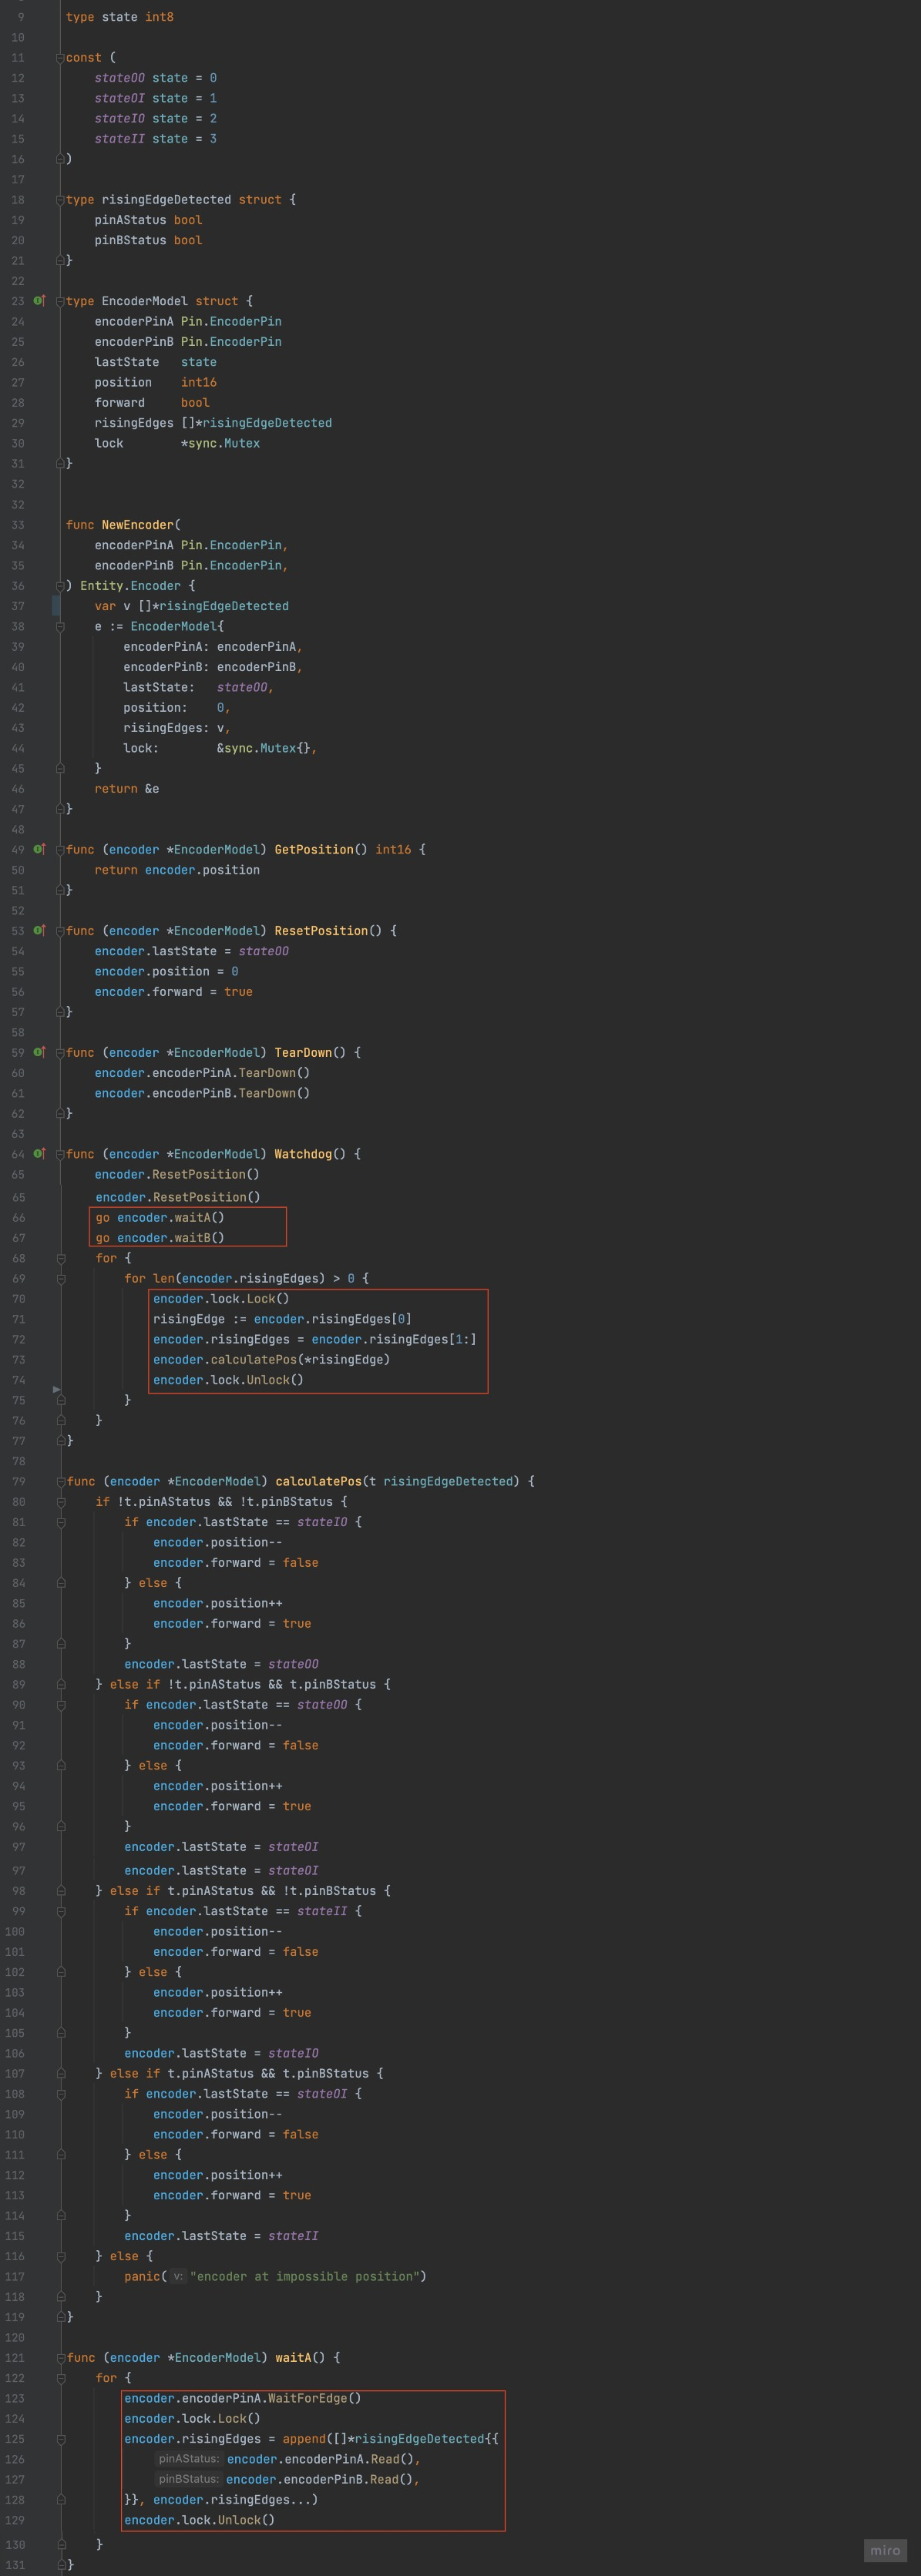
\includegraphics[height=0.95\textheight]{./part/Ejecucion/Seguimiento/PidControl/img/PFM - Encoder}
    \caption{EncoderAdapter.go}\label{fig:EncoderAdapter}
\end{figure}